\documentclass[tikz,border=6pt]{standalone}
% Shared preamble of the standalone figures: fonts as in the decks, the TikZ
% libraries, the notation, and the styles.
\usepackage[T1]{fontenc}
\usepackage[utf8]{inputenc}
\usepackage[sfdefault,lining]{FiraSans}
\usepackage{FiraMono}
\usepackage{amsmath}
\usetikzlibrary{positioning,arrows.meta,calc,shapes.misc,fit,backgrounds,
                decorations.pathreplacing,patterns,matrix}
% Notation for the MACE4D figures.
%
% Every parameter, symbol, default value, and constant that a figure shows is
% a macro here, so that the figures change from code names to symbols, or
% follow a change of a default, by editing this file alone.
%
%   \codenamestrue   renders each parameter as its code name (current setting)
%   \codenamesfalse  renders the symbolic form
%
% \sym{code name}{symbol} is the switch every parameter macro uses.  A
% parameter that exists on both models carries its owner in code mode.

\newif\ifcodenames
\codenamestrue

\providecommand{\code}[1]{\texttt{#1}}
\newcommand{\sym}[2]{\ifcodenames\code{#1}\else\ensuremath{#2}\fi}
\newcommand{\ctmodel}{\code{ct\_model}}
\newcommand{\macemodel}{\code{MACE4DModel}}
% A key line "code name <-> symbol", shown in code mode only.
\newcommand{\keyline}[2]{\ifcodenames#1~\ensuremath{\leftrightarrow}~\ensuremath{#2}\fi}

% ------------------------------------------------------------ math symbols
% These are always symbolic; the formulas use them, and the key lines tie
% them to the code names.
\newcommand{\symSigY}{\sigma_y}
\newcommand{\symSigProx}{\sigma_p}
\newcommand{\symSigNoise}{\sigma_n}
\newcommand{\symSigX}{\sigma_x}
\newcommand{\symSharpness}{s}
\newcommand{\symBeta}[1]{\beta_{#1}}
\newcommand{\symRho}{\rho}
\newcommand{\symNbrWeightTime}{b_t}
\newcommand{\symNumFrames}{T}
\newcommand{\symFramesPerRotation}{P}
\newcommand{\symOverlap}{f}

% ------------------------------------------------------------------ objects
\newcommand{\frameCube}[1]{\ensuremath{C_{#1}}}          % frame t of the 4D image
\newcommand{\fourD}{\ensuremath{x}}                      % the 4D image
\newcommand{\initImage}{\ensuremath{x^{0}}}              % the initial 4D image
\newcommand{\sinoFrame}[1]{\ensuremath{y_{#1}}}          % the views of frame t
\newcommand{\weightsFrame}[1]{\ensuremath{\Lambda_{#1}}} % the weights of frame t
\newcommand{\projFrame}[1]{\ensuremath{A_{#1}}}          % the frame model
\newcommand{\proxAgent}[1]{\ensuremath{F_{#1}}}          % the prox map of frame t
\newcommand{\dataFitAgent}{\ensuremath{F}}               % all frames' prox maps as one agent
\newcommand{\orientXY}{\sym{XY-t}{\mathrm{XY}t}}
\newcommand{\orientYZ}{\sym{YZ-t}{\mathrm{YZ}t}}
\newcommand{\orientXZ}{\sym{XZ-t}{\mathrm{XZ}t}}
\newcommand{\denoiser}[1]{\ensuremath{G_{#1}}}           % \denoiser{\orientXY}
\newcommand{\stateW}[1]{\ensuremath{W_{#1}}}             % the loop's input to agent k
\newcommand{\outX}[1]{\ensuremath{X_{#1}}}               % the output of agent k
\newcommand{\avgZ}{\ensuremath{z}}
\newcommand{\xbar}{\ensuremath{\bar{x}}}
\newcommand{\filterMatrix}{\sym{filter\_matrix}{H}}
\newcommand{\genInit}{\code{'init'}}                     % the generator of the partitions
\newcommand{\genIteration}{the iteration number}          % the generator of the subset order

% --------------------------------------------- parameters and their defaults
% Scan and frames (constructor arguments of MACE4DModel)
\newcommand{\pFramesPerRotation}{\sym{frames\_per\_rotation}{\symFramesPerRotation}}
\newcommand{\defFramesPerRotation}{6}
\newcommand{\pFrameOverlapFactor}{\sym{frame\_overlap\_factor}{\symOverlap}}
\newcommand{\defFrameOverlapFactor}{2.0}
\newcommand{\pNumFrames}{\sym{num\_frames}{\symNumFrames}}
\newcommand{\defNumFrames}{all}

% Set on ct_model; reach the frame models
\newcommand{\pSnrDb}{\sym{snr\_db}{\mathrm{SNR}_{\mathrm{dB}}}}
\newcommand{\defSnrDb}{30}
\newcommand{\pSharpnessCt}{\sym{ct\_model.sharpness}{\symSharpness_{\mathrm{ct}}}}
\newcommand{\defSharpnessCt}{1.0}
\newcommand{\pSigmaProxCt}{\sym{ct\_model.sigma\_prox}{\symSigProx^{\mathrm{ct}}}}
\newcommand{\pSigmaXCt}{\sym{ct\_model.sigma\_x}{\symSigX^{\mathrm{ct}}}}
\newcommand{\pPQTCt}{\sym{ct\_model.p, q, T}{(p, q, T)_{\mathrm{ct}}}}
\newcommand{\pSigmaY}{\sym{sigma\_y}{\symSigY}}

% Set on MACE4DModel
\newcommand{\pSigmaProxMace}{\sym{MACE4DModel.sigma\_prox}{\symSigProx}}
\newcommand{\defSigmaProxMace}{None (estimated per frame)}
\newcommand{\pSigmaNoise}{\sym{sigma\_noise}{\symSigNoise}}
\newcommand{\defSigmaNoise}{None (estimated)}
\newcommand{\pSigmaXMace}{\sym{MACE4DModel.sigma\_x}{\symSigX}}
\newcommand{\defSigmaXMace}{estimated}
\newcommand{\pSharpnessMace}{\sym{MACE4DModel.sharpness}{\symSharpness}}
\newcommand{\defSharpnessMace}{0.0}
\newcommand{\pPQTMace}{\sym{MACE4DModel.p, q, T}{(p, q, T)}}
\newcommand{\defPQT}{2.0, 1.2, 1.0}
\newcommand{\pNbrWeightTime}{\sym{nbr\_weight\_time}{\symNbrWeightTime}}
\newcommand{\defNbrWeightTime}{1.0}
\newcommand{\pMacePriorWeight}{\sym{mace\_prior\_weight}{\beta}}
\newcommand{\defMacePriorWeight}{0.5}
\newcommand{\pRhoMann}{\sym{rho\_mann}{\symRho}}
\newcommand{\defRhoMann}{0.5}
\newcommand{\pProxNumIterations}{\sym{prox\_num\_iterations}{N_p}}
\newcommand{\defProxNumIterations}{3}
\newcommand{\pProxPartitionAdvance}{\sym{prox\_partition\_advance}{a}}
\newcommand{\defProxPartitionAdvance}{1.0}
\newcommand{\pProxWarmStart}{\code{prox\_warm\_start}}
\newcommand{\defProxWarmStart}{True}
\newcommand{\pProxStopThreshold}{\code{prox\_stop\_threshold}}
\newcommand{\defProxStopThreshold}{0.02}
\newcommand{\pDenoiserWarmStart}{\code{denoiser\_warm\_start}}
\newcommand{\defDenoiserWarmStart}{False}
\newcommand{\pDenoiseSlabGb}{\code{denoise\_slab\_gb}}
\newcommand{\defDenoiseSlabGb}{2.0}
\newcommand{\pDejitter}{\code{dejitter}}
\newcommand{\defDejitter}{True}
\newcommand{\pDevicePool}{\code{set\_device\_pool}}
\newcommand{\pNumDevicesEnv}{\code{MBIRTORCH\_NUM\_DEVICES}}

% Arguments of MACE4DModel.recon
\newcommand{\pMaxIterations}{\sym{max\_iterations}{N}}
\newcommand{\defMaxIterations}{10}
\newcommand{\pStopThreshold}{\code{stop\_threshold\_change\_pct}}
\newcommand{\defStopThreshold}{0.2}
\newcommand{\pSeed}{\code{seed}}
\newcommand{\defSeed}{None}
\newcommand{\pInitRecon}{\code{init\_recon}}
\newcommand{\pInitDir}{\code{init\_dir}}

% ---------------------------------------------------------------- constants
\newcommand{\cInitIterations}{15}        % iterations of the per-frame initial image
\newcommand{\cDenoiseMaxIterations}{15}  % iterations per denoised volume, at most
\newcommand{\cDenoiseStopPct}{0.05}      % percent change that stops a denoised volume
\newcommand{\cSigmaXFactor}{0.2}         % sigma_x and sigma_prox estimates: factor * 2^sharpness * std
\newcommand{\cSigmaXFloor}{10^{-6}}      % floor of the denoiser sigma_x estimate
\newcommand{\cSigmaXBase}{1.0}           % base default of sigma_x when no estimate runs
\newcommand{\cDenoiseSubsets}{16}        % pixel subsets of a denoiser partition, at most
\newcommand{\cPixelsPerSubset}{64}       % fewer pixels per subset than this and the count drops

% ------------------------------------------- symbols the figures use inline
\newcommand{\symPriorWeight}{\ensuremath{w}}    % the value of the prior weight
\newcommand{\symFilterMatrix}{\ensuremath{H}}   % the temporal filter
\newcommand{\symFrameIndex}{\ensuremath{t}}
\newcommand{\symNumDevices}{\ensuremath{n}}     % the size of the device pool
\newcommand{\degsym}{\ensuremath{^{\circ}}}
% Argument values of the device pool selector
\newcommand{\valNone}{\code{None}}
\newcommand{\valCpu}{\code{'cpu'}}
\newcommand{\valGpu}{\code{'gpu'}}
% Derived defaults, in degrees (integers; add rounding if a default ever gives a fraction)
\newcommand{\defFrameStepDeg}{\pgfmathparse{int(360/\defFramesPerRotation)}\pgfmathresult}
\newcommand{\defFrameSpanDeg}{\pgfmathparse{int(\defFrameOverlapFactor*360/\defFramesPerRotation)}\pgfmathresult}
% Axis labels of the 4D image
\newcommand{\axisT}{\ensuremath{t}}
\newcommand{\axisX}{\ensuremath{x}}
\newcommand{\axisY}{\ensuremath{y}}
\newcommand{\axisZ}{\ensuremath{z}}

% Colors and TikZ styles shared by the MACE4D figures.
%
% Blue is the data-fit side, green the priors, amber the consensus state.
% A solid arrow carries a value the user set; a dashed arrow carries an
% estimate.  \cube draws one frame of the 4D image.

\definecolor{datafitBlue}{HTML}{3D6B99}
\definecolor{priorGreen}{HTML}{2E7D32}
\definecolor{stateAmber}{HTML}{B26B1F}
\definecolor{warnRed}{HTML}{A23B3B}
\definecolor{inkGray}{HTML}{5A5A5A}
\definecolor{lineGray}{HTML}{9A9A9A}
\definecolor{paleBlue}{HTML}{E3ECF5}
\definecolor{paleGreen}{HTML}{E4F0E4}
\definecolor{paleAmber}{HTML}{F5EBDD}
\definecolor{paleGray}{HTML}{F0F0F0}

\tikzset{
  every node/.style={font=\small},
  box/.style={draw, rounded corners=3pt, thick, align=center, inner sep=5pt,
              minimum height=8mm},
  datafit/.style={box, draw=datafitBlue, fill=paleBlue},
  prior/.style={box, draw=priorGreen, fill=paleGreen},
  state/.style={box, draw=stateAmber, fill=paleAmber},
  plain/.style={box, draw=lineGray, fill=paleGray},
  note/.style={font=\footnotesize, text=inkGray, align=left},
  notebox/.style={note, draw=lineGray, rounded corners=2pt, inner sep=4pt,
                  fill=white},
  param/.style={font=\footnotesize, align=left},
  title/.style={font=\bfseries, align=left},
  setarrow/.style={-{Stealth[length=2mm]}, thick},
  estarrow/.style={-{Stealth[length=2mm]}, thick, dashed, inkGray},
  flow/.style={-{Stealth[length=2mm]}, semithick},
  flowblue/.style={flow, datafitBlue},
  flowgreen/.style={flow, priorGreen},
  flowamber/.style={flow, stateAmber},
  cut/.style={-{Stealth[length=1.5mm]}, thin, inkGray},
  cubeFront/.style={fill=white, draw=black!70, thin},
  cubeTop/.style={fill=black!8, draw=black!70, thin},
  cubeSide/.style={fill=black!20, draw=black!70, thin},
}

% \cube{x}{y}{size}{label}: a cube whose front face has its lower left
% corner at (x, y) and side length size, with a label on the front face.
\newcommand{\cube}[4]{%
  \begin{scope}[shift={(#1,#2)}]
    \pgfmathsetmacro{\cubeDepth}{0.35*#3}
    \draw[cubeTop] (0,#3) -- (\cubeDepth,#3+\cubeDepth) -- (#3+\cubeDepth,#3+\cubeDepth) -- (#3,#3) -- cycle;
    \draw[cubeSide] (#3,0) -- (#3+\cubeDepth,\cubeDepth) -- (#3+\cubeDepth,#3+\cubeDepth) -- (#3,#3) -- cycle;
    \draw[cubeFront] (0,0) rectangle (#3,#3);
    \node at (0.5*#3,0.5*#3) {#4};
  \end{scope}}

% \arrowkey{x}{y}: the legend of the two arrow kinds, anchored at (x, y).
\newcommand{\arrowkey}[2]{%
  \draw[setarrow] (#1,#2) -- ++(1,0) node[note, right] {set by the user};
  \draw[estarrow] (#1,#2-0.45) -- ++(1,0) node[note, right] {estimated from the data};}


% keep the short labels unbroken
\hyphenpenalty=10000 \exhyphenpenalty=10000
\begin{document}
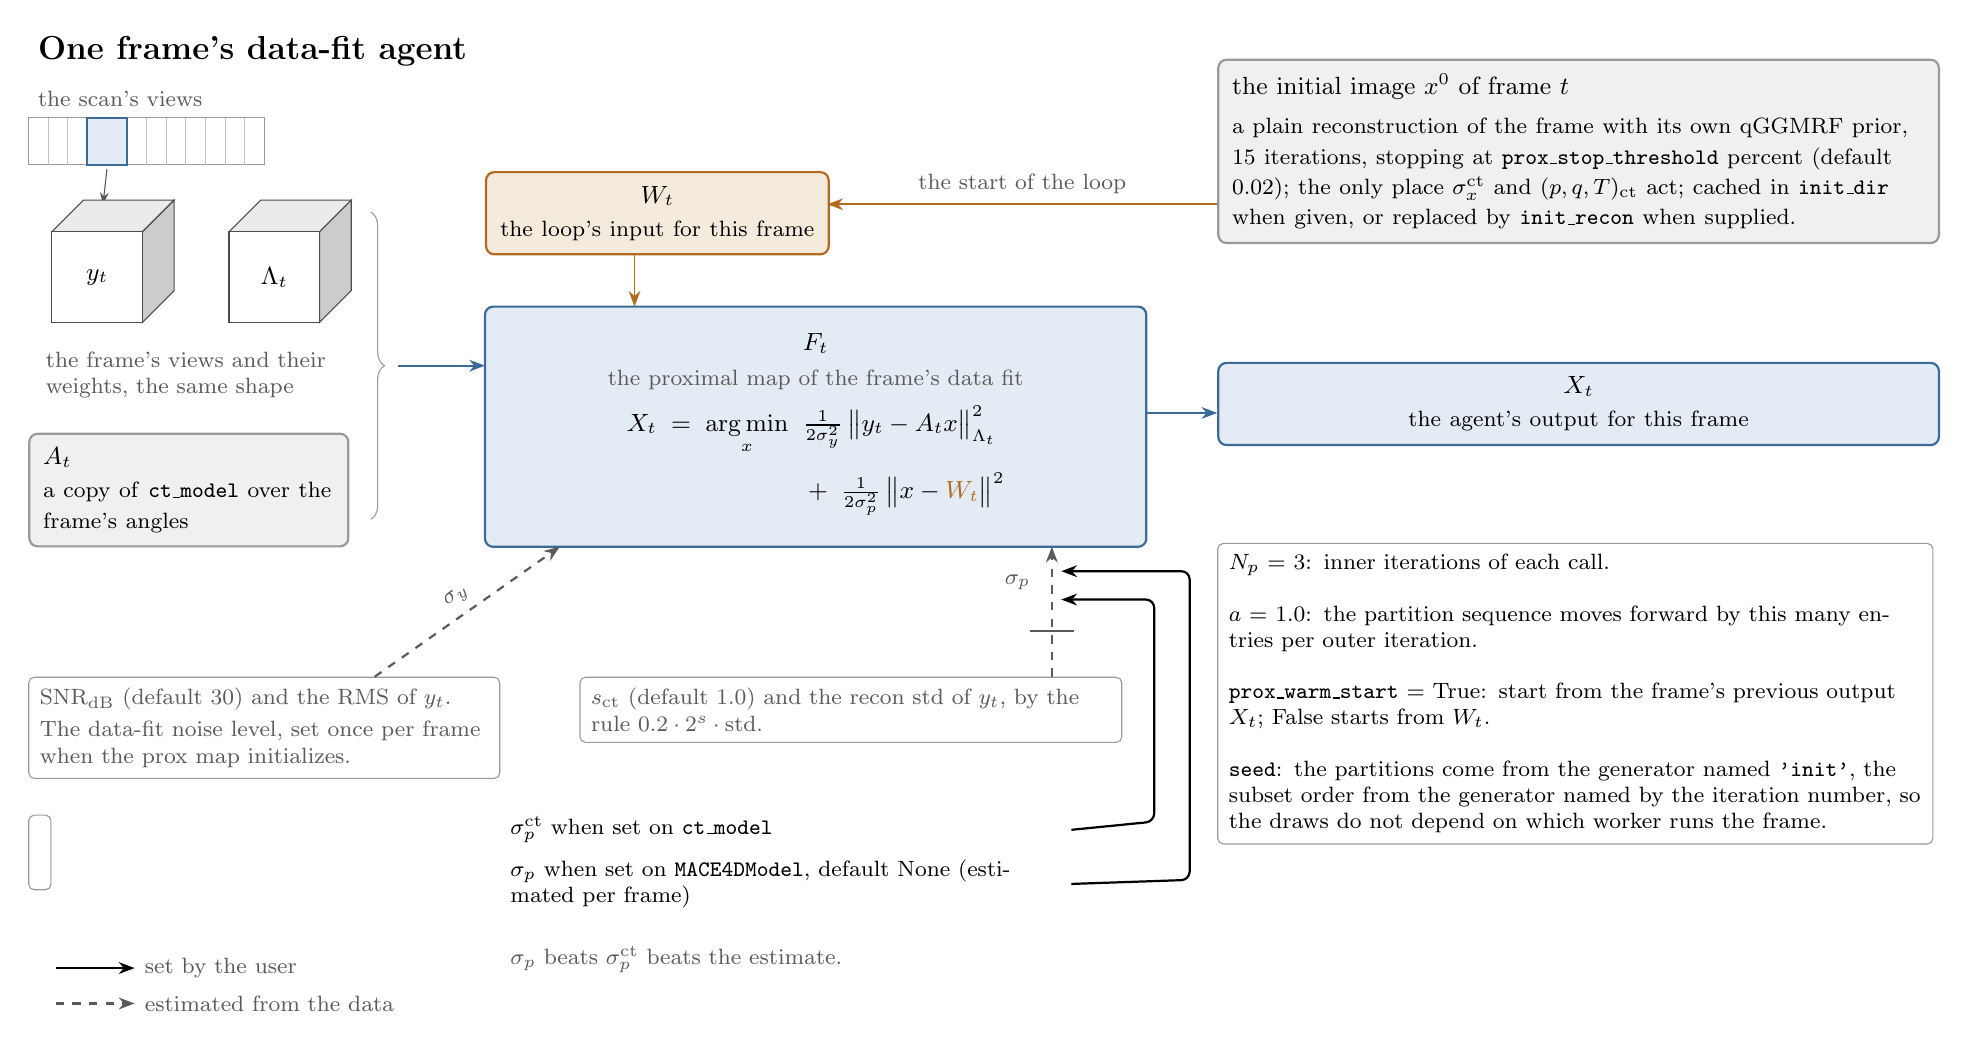
\begin{tikzpicture}

% ------------------------------------------------------------------- title
\node[title, anchor=north west] at (0.2,13.35) {\large One frame's data-fit agent};

% ------------------------------------- left: the inputs that belong to frame t
% the scan's views, with the frame's angles marked
\node[note, anchor=south west] at (0.2,12.22) {the scan's views};
\draw[thin, draw=lineGray, fill=white] (0.2,11.60) rectangle (3.20,12.20);
\foreach \i in {1,...,11} {\draw[lineGray!60, very thin] (0.2+\i*0.25,11.60) -- ++(0,0.60);}
\draw[thick, draw=datafitBlue, fill=paleBlue] (0.95,11.60) rectangle (1.45,12.20);
\draw[cut] (1.20,11.55) -- (1.15,11.10);

% the frame's own views and weights
\cube{0.50}{9.60}{1.15}{\sinoFrame{t}}
\cube{2.75}{9.60}{1.15}{\weightsFrame{t}}
\node[note, anchor=north west, text width=4.20cm] at (0.30,9.35)
  {the frame's views and their weights, the same shape};

% the frame's own projector
\node[plain, anchor=north west, text width=3.70cm, align=left] at (0.20,8.20)
  {\projFrame{t}\\[1pt]{\footnotesize a copy of \ctmodel{} over the frame's angles}};

% the three inputs gathered into the agent
\draw[decorate, decoration={brace, amplitude=5pt}, lineGray]
  (4.55,11.00) -- (4.55,7.10);
\draw[flowblue] (4.90,9.05) -- (6.00,9.05);

% ------------------------------------------------- center: the agent itself
\coordinate (agentSW) at (6.00,6.75);
\coordinate (agentNE) at (14.40,9.80);
\node[datafit, fit={(agentSW) (agentNE)}, inner sep=0pt] (agent) {};
\node[anchor=north] at (10.20,9.58) {\textbf{\proxAgent{t}}};
\node[note, anchor=north, align=center] at (10.20,9.12)
  {the proximal map of the frame's data fit};
\node[anchor=north] at (10.20,8.66)
  {$\begin{aligned}
     \outX{t} \;=\; \operatorname*{arg\,min}_{x}\;\;
       & \tfrac{1}{2\symSigY^{2}}\,\big\|\sinoFrame{t}-\projFrame{t}x\big\|^{2}_{\weightsFrame{t}}\\[3pt]
       & +\;\tfrac{1}{2\symSigProx^{2}}\,\big\|x-\textcolor{stateAmber}{\stateW{t}}\big\|^{2}
   \end{aligned}$};

% the loop's input for this frame
\node[state, anchor=south west, text width=4.00cm, align=center] (w) at (6.00,10.45)
  {\stateW{t}\\[1pt]{\footnotesize the loop's input for this frame}};
\draw[flowamber] (7.90,10.45) -- (7.90,9.80);

% ------------------------------------------- right: start, output, settings
\node[plain, anchor=north west, text width=8.80cm, align=left] (init) at (15.30,12.95)
  {the initial image \initImage{} of frame $t$\\[3pt]
   {\footnotesize a plain reconstruction of the frame with its own qGGMRF prior,
    \cInitIterations{} iterations, stopping at \pProxStopThreshold{} percent
    (default \defProxStopThreshold); the only place \pSigmaXCt{} and \pPQTCt{}
    act; cached in \pInitDir{} when given, or replaced by \pInitRecon{} when
    supplied.}};
\draw[flowamber] (15.30,11.10) -- (10.35,11.10)
  node[note, midway, above] {the start of the loop};

\node[datafit, anchor=north west, text width=8.80cm, align=center] (out) at (15.30,9.10)
  {\outX{t}\\[1pt]{\footnotesize the agent's output for this frame}};
\draw[flowblue] (14.40,8.45) -- (15.30,8.45);

\node[param, draw=lineGray, rounded corners=2pt, fill=white, inner sep=4pt,
      anchor=north west, text width=8.80cm] (par) at (15.30,6.80)
  {\pProxNumIterations{} = \defProxNumIterations: inner iterations of each call.\\[9pt]
   \pProxPartitionAdvance{} = \defProxPartitionAdvance: the partition sequence moves
     forward by this many entries per outer iteration.\\[9pt]
   \pProxWarmStart{} = \defProxWarmStart: start from the frame's previous output
     \outX{t}; False starts from \stateW{t}.\\[9pt]
   \pSeed{}: the partitions come from the generator named \genInit{}, the subset order
     from the generator named by \genIteration{}, so the draws do not depend on which
     worker runs the frame.};

% ------------------------------------- bottom: where the two strengths come from
\node[notebox, anchor=north west, text width=5.70cm] (sy) at (0.20,5.10)
  {\pSnrDb{} (default \defSnrDb) and the RMS of \sinoFrame{t}.\\[2pt]
   The data-fit noise level, set once per frame when the prox map initializes.};
\draw[estarrow] (4.60,5.10) -- (6.95,6.75)
  node[note, midway, above, sloped] {$\symSigY$};

\node[notebox, anchor=north west, text width=6.60cm] (sp) at (7.20,5.10)
  {\pSharpnessCt{} (default \defSharpnessCt) and the recon std of \sinoFrame{t},
   by the rule $\cSigmaXFactor \cdot 2^{\symSharpness} \cdot \mathrm{std}$.};
\draw[estarrow] (13.20,5.10) -- (13.20,6.75);
\node[note, anchor=east] at (13.05,6.30) {$\symSigProx$};

% two settings that replace the estimate: they cut it and take its place
\draw[thick, inkGray] (12.92,5.68) -- (13.48,5.68);
\node[param, anchor=north west, text width=7.00cm] (ovrA) at (6.20,3.45)
  {\pSigmaProxCt{} when set on \ctmodel{}};
\node[param, anchor=north west, text width=7.00cm] (ovrB) at (6.20,2.90)
  {\pSigmaProxMace{} when set on \macemodel{}, default \defSigmaProxMace};
\draw[setarrow, rounded corners=3pt]
  (ovrA.east) -- (14.50,3.26) -- (14.50,6.08) -- (13.32,6.08);
\draw[setarrow, rounded corners=3pt]
  (ovrB.east) -- (14.95,2.52) -- (14.95,6.44) -- (13.32,6.44);
\node[note, anchor=north west, text width=8.60cm] at (6.20,1.80)
  {\pSigmaProxMace{} beats \pSigmaProxCt{} beats the estimate.};

% ---------------------------------------- bottom left: the keys to the figure
\node[notebox, anchor=north west] at (0.20,3.35)
  {\keyline{\pSigmaY}{\symSigY}\\
   \keyline{\pSigmaProxMace}{\symSigProx}\\
   \keyline{\pSharpnessCt}{\symSharpness}};
\arrowkey{0.55}{1.40}

\end{tikzpicture}
\end{document}
